\documentclass[1p]{elsarticle_modified}
%\bibliographystyle{elsarticle-num}

%\usepackage[colorlinks]{hyperref}
%\usepackage{abbrmath_seonhwa} %\Abb, \Ascr, \Acal ,\Abf, \Afrak
\usepackage{amsfonts}
\usepackage{amssymb}
\usepackage{amsmath}
\usepackage{amsthm}
\usepackage{scalefnt}
\usepackage{amsbsy}
\usepackage{kotex}
\usepackage{caption}
\usepackage{subfig}
\usepackage{color}
\usepackage{graphicx}
\usepackage{xcolor} %% white, black, red, green, blue, cyan, magenta, yellow
\usepackage{float}
\usepackage{setspace}
\usepackage{hyperref}

\usepackage{tikz}
\usetikzlibrary{arrows}

\usepackage{multirow}
\usepackage{array} % fixed length table
\usepackage{hhline}

%%%%%%%%%%%%%%%%%%%%%
\makeatletter
\renewcommand*\env@matrix[1][\arraystretch]{%
	\edef\arraystretch{#1}%
	\hskip -\arraycolsep
	\let\@ifnextchar\new@ifnextchar
	\array{*\c@MaxMatrixCols c}}
\makeatother %https://tex.stackexchange.com/questions/14071/how-can-i-increase-the-line-spacing-in-a-matrix
%%%%%%%%%%%%%%%

\usepackage[normalem]{ulem}

\newcommand{\msout}[1]{\ifmmode\text{\sout{\ensuremath{#1}}}\else\sout{#1}\fi}
%SOURCE: \msout is \stkout macro in https://tex.stackexchange.com/questions/20609/strikeout-in-math-mode

\newcommand{\cancel}[1]{
	\ifmmode
	{\color{red}\msout{#1}}
	\else
	{\color{red}\sout{#1}}
	\fi
}

\newcommand{\add}[1]{
	{\color{blue}\uwave{#1}}
}

\newcommand{\replace}[2]{
	\ifmmode
	{\color{red}\msout{#1}}{\color{blue}\uwave{#2}}
	\else
	{\color{red}\sout{#1}}{\color{blue}\uwave{#2}}
	\fi
}

\newcommand{\Sol}{\mathcal{S}} %segment
\newcommand{\D}{D} %diagram
\newcommand{\A}{\mathcal{A}} %arc


%%%%%%%%%%%%%%%%%%%%%%%%%%%%%5 test

\def\sl{\operatorname{\textup{SL}}(2,\Cbb)}
\def\psl{\operatorname{\textup{PSL}}(2,\Cbb)}
\def\quan{\mkern 1mu \triangleright \mkern 1mu}

\theoremstyle{definition}
\newtheorem{thm}{Theorem}[section]
\newtheorem{prop}[thm]{Proposition}
\newtheorem{lem}[thm]{Lemma}
\newtheorem{ques}[thm]{Question}
\newtheorem{cor}[thm]{Corollary}
\newtheorem{defn}[thm]{Definition}
\newtheorem{exam}[thm]{Example}
\newtheorem{rmk}[thm]{Remark}
\newtheorem{alg}[thm]{Algorithm}

\newcommand{\I}{\sqrt{-1}}
\begin{document}

%\begin{frontmatter}
%
%\title{Boundary parabolic representations of knots up to 8 crossings}
%
%%% Group authors per affiliation:
%\author{Yunhi Cho} 
%\address{Department of Mathematics, University of Seoul, Seoul, Korea}
%\ead{yhcho@uos.ac.kr}
%
%
%\author{Seonhwa Kim} %\fnref{s_kim}}
%\address{Center for Geometry and Physics, Institute for Basic Science, Pohang, 37673, Korea}
%\ead{ryeona17@ibs.re.kr}
%
%\author{Hyuk Kim}
%\address{Department of Mathematical Sciences, Seoul National University, Seoul 08826, Korea}
%\ead{hyukkim@snu.ac.kr}
%
%\author{Seokbeom Yoon}
%\address{Department of Mathematical Sciences, Seoul National University, Seoul, 08826,  Korea}
%\ead{sbyoon15@snu.ac.kr}
%
%\begin{abstract}
%We find all boundary parabolic representation of knots up to 8 crossings.
%
%\end{abstract}
%\begin{keyword}
%    \MSC[2010] 57M25 
%\end{keyword}
%
%\end{frontmatter}

%\linenumbers
%\tableofcontents
%
\newcommand\colored[1]{\textcolor{white}{\rule[-0.35ex]{0.8em}{1.4ex}}\kern-0.8em\color{red} #1}%
%\newcommand\colored[1]{\textcolor{white}{ #1}\kern-2.17ex	\textcolor{white}{ #1}\kern-1.81ex	\textcolor{white}{ #1}\kern-2.15ex\color{red}#1	}

{\Large $\underline{10_{103}~(K10a_{105})}$}

\setlength{\tabcolsep}{10pt}
\renewcommand{\arraystretch}{1.6}
\vspace{1cm}\begin{tabular}{m{100pt}>{\centering\arraybackslash}m{274pt}}
\multirow{5}{120pt}{
	\centering
	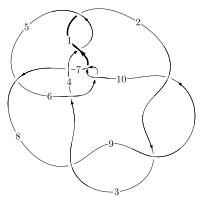
\includegraphics[width=112pt]{../../../GIT/diagram.site/Diagrams/png/187_10_103.png}\\
\ \ \ A knot diagram\footnotemark}&
\allowdisplaybreaks
\textbf{Linearized knot diagam} \\
\cline{2-2}
 &
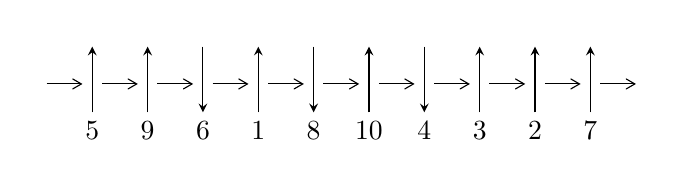
\begin{tikzpicture}[x=20pt, y=17pt]
	% nodes
	\node (C0) at (0, 0) {};
	\node (C1) at (1, 0) {};
	\node (C1U) at (1, +1) {};
	\node (C1D) at (1, -1) {5};

	\node (C2) at (2, 0) {};
	\node (C2U) at (2, +1) {};
	\node (C2D) at (2, -1) {9};

	\node (C3) at (3, 0) {};
	\node (C3U) at (3, +1) {};
	\node (C3D) at (3, -1) {6};

	\node (C4) at (4, 0) {};
	\node (C4U) at (4, +1) {};
	\node (C4D) at (4, -1) {1};

	\node (C5) at (5, 0) {};
	\node (C5U) at (5, +1) {};
	\node (C5D) at (5, -1) {8};

	\node (C6) at (6, 0) {};
	\node (C6U) at (6, +1) {};
	\node (C6D) at (6, -1) {10};

	\node (C7) at (7, 0) {};
	\node (C7U) at (7, +1) {};
	\node (C7D) at (7, -1) {4};

	\node (C8) at (8, 0) {};
	\node (C8U) at (8, +1) {};
	\node (C8D) at (8, -1) {3};

	\node (C9) at (9, 0) {};
	\node (C9U) at (9, +1) {};
	\node (C9D) at (9, -1) {2};

	\node (C10) at (10, 0) {};
	\node (C10U) at (10, +1) {};
	\node (C10D) at (10, -1) {7};
	\node (C11) at (11, 0) {};

	% arrows
	\draw[->,>={angle 60}]
	(C0) edge (C1) (C1) edge (C2) (C2) edge (C3) (C3) edge (C4) (C4) edge (C5) (C5) edge (C6) (C6) edge (C7) (C7) edge (C8) (C8) edge (C9) (C9) edge (C10) (C10) edge (C11) ;	\draw[->,>=stealth]
	(C1D) edge (C1U) (C2D) edge (C2U) (C3U) edge (C3D) (C4D) edge (C4U) (C5U) edge (C5D) (C6D) edge (C6U) (C7U) edge (C7D) (C8D) edge (C8U) (C9D) edge (C9U) (C10D) edge (C10U) ;
	\end{tikzpicture} \\
\hhline{~~} \\& 
\textbf{Solving Sequence} \\ \cline{2-2} 
 &
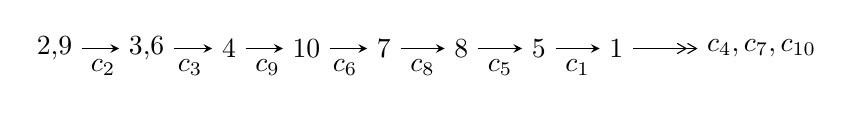
\begin{tikzpicture}[x=28pt, y=7pt]
	% node
	\node (A0) at (-1/8, 0) {2,9};
	\node (A1) at (17/16, 0) {3,6};
	\node (A2) at (17/8, 0) {4};
	\node (A3) at (25/8, 0) {10};
	\node (A4) at (33/8, 0) {7};
	\node (A5) at (41/8, 0) {8};
	\node (A6) at (49/8, 0) {5};
	\node (A7) at (57/8, 0) {1};
	\node (C1) at (1/2, -1) {$c_{2}$};
	\node (C2) at (13/8, -1) {$c_{3}$};
	\node (C3) at (21/8, -1) {$c_{9}$};
	\node (C4) at (29/8, -1) {$c_{6}$};
	\node (C5) at (37/8, -1) {$c_{8}$};
	\node (C6) at (45/8, -1) {$c_{5}$};
	\node (C7) at (53/8, -1) {$c_{1}$};
	\node (A8) at (9, 0) {$c_{4},c_{7},c_{10}$};

	% edge
	\draw[->,>=stealth]	
	(A0) edge (A1) (A1) edge (A2) (A2) edge (A3) (A3) edge (A4) (A4) edge (A5) (A5) edge (A6) (A6) edge (A7) ;
	\draw[->>,>={angle 60}]	
	(A7) edge (A8);
\end{tikzpicture} \\ 

\end{tabular} \\

\footnotetext{
The image of knot diagram is generated by the software ``\textbf{Draw programme}" developed by Andrew Bartholomew(\url{http://www.layer8.co.uk/maths/draw/index.htm\#Running-draw}), where we modified some parts for our purpose(\url{https://github.com/CATsTAILs/LinksPainter}).
}\phantom \\ \newline 
\centering \textbf{Ideals for irreducible components\footnotemark of $X_{\text{par}}$} 
 
\begin{align*}
I^u_{1}&=\langle 
- u^{14}-7 u^{13}+\cdots+2 b+6,\;-3 u^{14}-17 u^{13}+\cdots+4 a+24,\;u^{15}+5 u^{14}+\cdots-22 u-4\rangle \\
I^u_{2}&=\langle 
- a^3 u- a^3+a^2 u+2 u^2 a+2 a^2+2 a u-3 u^2+4 b+a- u-7,\\
\phantom{I^u_{2}}&\phantom{= \langle  }- a^3 u^2+a^4+a^3 u+a^2 u^2-2 a^3+6 u^2 a-2 a^2-3 a u+7 u^2+11 a-3 u+17,\;u^3+2 u+1\rangle \\
I^u_{3}&=\langle 
- u^6+2 u^5-4 u^4+4 u^3-3 u^2+b+u,\;u^4-2 u^3+3 u^2+a-3 u+1,\;u^7- u^6+4 u^5-3 u^4+4 u^3-3 u^2-1\rangle \\
I^u_{4}&=\langle 
- u^3 a+u^2 a- u^3-2 a u+u^2+b+a- u+1,\;u^3 a+u^2 a-2 u^3+a^2+u^2- u,\;u^4- u^3+2 u^2-2 u+1\rangle \\
I^u_{5}&=\langle 
b- u,\;a,\;u^4- u^3+2 u^2-2 u+1\rangle \\
I^u_{6}&=\langle 
u^3-2 u^2+b+2 u-1,\;- u^2+a+1,\;u^4- u^3+2 u^2-2 u+1\rangle \\
I^u_{7}&=\langle 
b+1,\;a,\;u+1\rangle \\
\\
\end{align*}
\raggedright * 7 irreducible components of $\dim_{\mathbb{C}}=0$, with total 51 representations.\\
\footnotetext{All coefficients of polynomials are rational numbers. But the coefficients are sometimes approximated in decimal forms when there is not enough margin.}
\newpage
\renewcommand{\arraystretch}{1}
\centering \section*{I. $I^u_{1}= \langle - u^{14}-7 u^{13}+\cdots+2 b+6,\;-3 u^{14}-17 u^{13}+\cdots+4 a+24,\;u^{15}+5 u^{14}+\cdots-22 u-4 \rangle$}
\flushleft \textbf{(i) Arc colorings}\\
\begin{tabular}{m{7pt} m{180pt} m{7pt} m{180pt} }
\flushright $a_{2}=$&$\begin{pmatrix}1\\0\end{pmatrix}$ \\
\flushright $a_{9}=$&$\begin{pmatrix}0\\u\end{pmatrix}$ \\
\flushright $a_{3}=$&$\begin{pmatrix}1\\- u^2\end{pmatrix}$ \\
\flushright $a_{6}=$&$\begin{pmatrix}\frac{3}{4} u^{14}+\frac{17}{4} u^{13}+\cdots-\frac{107}{4} u-6\\\frac{1}{2} u^{14}+\frac{7}{2} u^{13}+\cdots-\frac{25}{2} u-3\end{pmatrix}$ \\
\flushright $a_{4}=$&$\begin{pmatrix}\frac{1}{2} u^{13}+\frac{3}{2} u^{12}+\cdots+\frac{13}{2} u+\frac{5}{2}\\\frac{1}{2} u^{14}+\frac{5}{2} u^{13}+\cdots-\frac{33}{2} u^2-\frac{7}{2} u\end{pmatrix}$ \\
\flushright $a_{10}=$&$\begin{pmatrix}u\\u\end{pmatrix}$ \\
\flushright $a_{7}=$&$\begin{pmatrix}-\frac{1}{4} u^{14}-\frac{3}{4} u^{13}+\cdots-\frac{67}{4} u-4\\-\frac{1}{2} u^{14}-\frac{3}{2} u^{13}+\cdots-\frac{5}{2} u-1\end{pmatrix}$ \\
\flushright $a_{8}=$&$\begin{pmatrix}- u\\u^3+u\end{pmatrix}$ \\
\flushright $a_{5}=$&$\begin{pmatrix}\frac{3}{4} u^{14}+\frac{13}{4} u^{13}+\cdots-\frac{59}{4} u-4\\\frac{1}{2} u^{14}+\frac{3}{2} u^{13}+\cdots-\frac{5}{2} u-1\end{pmatrix}$ \\
\flushright $a_{1}=$&$\begin{pmatrix}-\frac{1}{2} u^{13}-\frac{5}{2} u^{12}+\cdots+\frac{19}{2} u+\frac{5}{2}\\-\frac{1}{2} u^{14}-\frac{5}{2} u^{13}+\cdots+\frac{23}{2} u+2\end{pmatrix}$\\&\end{tabular}
\flushleft \textbf{(ii) Obstruction class $= -1$}\\~\\
\flushleft \textbf{(iii) Cusp Shapes $= -4 u^{14}-17 u^{13}-63 u^{12}-150 u^{11}-301 u^{10}-461 u^9-582 u^8-556 u^7-394 u^6-135 u^5+61 u^4+145 u^3+106 u^2+46 u+6$}\\~\\
\newpage\renewcommand{\arraystretch}{1}
\flushleft \textbf{(iv) u-Polynomials at the component}\newline \\
\begin{tabular}{m{50pt}|m{274pt}}
Crossings & \hspace{64pt}u-Polynomials at each crossing \\
\hline $$\begin{aligned}c_{1},c_{4},c_{6}\\c_{10}\end{aligned}$$&$\begin{aligned}
&u^{15}-5 u^{13}+12 u^{11}+u^{10}-13 u^9- u^8+7 u^7-2 u^6-2 u^5+6 u^4+4 u^3-1
\end{aligned}$\\
\hline $$\begin{aligned}c_{2},c_{8},c_{9}\end{aligned}$$&$\begin{aligned}
&u^{15}+5 u^{14}+\cdots-22 u-4
\end{aligned}$\\
\hline $$\begin{aligned}c_{3},c_{5}\end{aligned}$$&$\begin{aligned}
&u^{15}- u^{14}+\cdots+7 u-1
\end{aligned}$\\
\hline $$\begin{aligned}c_{7}\end{aligned}$$&$\begin{aligned}
&u^{15}+12 u^{14}+\cdots-352 u-64
\end{aligned}$\\
\hline
\end{tabular}\\~\\
\newpage\renewcommand{\arraystretch}{1}
\flushleft \textbf{(v) Riley Polynomials at the component}\newline \\
\begin{tabular}{m{50pt}|m{274pt}}
Crossings & \hspace{64pt}Riley Polynomials at each crossing \\
\hline $$\begin{aligned}c_{1},c_{4},c_{6}\\c_{10}\end{aligned}$$&$\begin{aligned}
&y^{15}-10 y^{14}+\cdots+12 y^2-1
\end{aligned}$\\
\hline $$\begin{aligned}c_{2},c_{8},c_{9}\end{aligned}$$&$\begin{aligned}
&y^{15}+15 y^{14}+\cdots+12 y-16
\end{aligned}$\\
\hline $$\begin{aligned}c_{3},c_{5}\end{aligned}$$&$\begin{aligned}
&y^{15}-7 y^{14}+\cdots+39 y-1
\end{aligned}$\\
\hline $$\begin{aligned}c_{7}\end{aligned}$$&$\begin{aligned}
&y^{15}+4 y^{14}+\cdots+15360 y-4096
\end{aligned}$\\
\hline
\end{tabular}\\~\\
\newpage\flushleft \textbf{(vi) Complex Volumes and Cusp Shapes}
$$\begin{array}{c|c|c}  
\text{Solutions to }I^u_{1}& \I (\text{vol} + \sqrt{-1}CS) & \text{Cusp shape}\\
 \hline 
\begin{aligned}
u &= -0.887920 + 0.390096 I \\
a &= -0.456559 + 0.349463 I \\
b &= \phantom{-}1.021850 + 0.430810 I\end{aligned}
 & \phantom{-}5.98098 - 9.46445 I & \phantom{-}7.81439 + 7.21994 I \\ \hline\begin{aligned}
u &= -0.887920 - 0.390096 I \\
a &= -0.456559 - 0.349463 I \\
b &= \phantom{-}1.021850 - 0.430810 I\end{aligned}
 & \phantom{-}5.98098 + 9.46445 I & \phantom{-}7.81439 - 7.21994 I \\ \hline\begin{aligned}
u &= -0.744334 + 0.885606 I \\
a &= \phantom{-}0.126989 + 0.717975 I \\
b &= -0.257749 - 0.301552 I\end{aligned}
 & \phantom{-}4.59236 + 3.90754 I & \phantom{-}6.20530 - 5.11964 I \\ \hline\begin{aligned}
u &= -0.744334 - 0.885606 I \\
a &= \phantom{-}0.126989 - 0.717975 I \\
b &= -0.257749 + 0.301552 I\end{aligned}
 & \phantom{-}4.59236 - 3.90754 I & \phantom{-}6.20530 + 5.11964 I \\ \hline\begin{aligned}
u &= \phantom{-}0.666897\phantom{ +0.000000I} \\
a &= -0.432662\phantom{ +0.000000I} \\
b &= \phantom{-}0.365528\phantom{ +0.000000I}\end{aligned}
 & \phantom{-}1.03900\phantom{ +0.000000I} & \phantom{-}11.4360\phantom{ +0.000000I} \\ \hline\begin{aligned}
u &= -0.12237 + 1.42140 I \\
a &= \phantom{-}1.69571 - 0.09050 I \\
b &= \phantom{-}2.22357 - 0.39328 I\end{aligned}
 & -6.94441 - 2.69912 I & -1.74572 + 0.84288 I \\ \hline\begin{aligned}
u &= -0.12237 - 1.42140 I \\
a &= \phantom{-}1.69571 + 0.09050 I \\
b &= \phantom{-}2.22357 + 0.39328 I\end{aligned}
 & -6.94441 + 2.69912 I & -1.74572 - 0.84288 I \\ \hline\begin{aligned}
u &= -0.41800 + 1.40303 I \\
a &= \phantom{-}1.190560 - 0.502109 I \\
b &= \phantom{-}1.52895 + 0.14725 I\end{aligned}
 & -2.92891 - 5.10870 I & \phantom{-}4.27958 + 4.78875 I \\ \hline\begin{aligned}
u &= -0.41800 - 1.40303 I \\
a &= \phantom{-}1.190560 + 0.502109 I \\
b &= \phantom{-}1.52895 - 0.14725 I\end{aligned}
 & -2.92891 + 5.10870 I & \phantom{-}4.27958 - 4.78875 I \\ \hline\begin{aligned}
u &= \phantom{-}0.00988 + 1.50056 I \\
a &= -0.858298 + 0.099548 I \\
b &= -1.290570 + 0.574441 I\end{aligned}
 & -4.75856 + 2.25763 I & \phantom{-}0.39685 - 3.44983 I\\
 \hline 
 \end{array}$$\newpage$$\begin{array}{c|c|c}  
\text{Solutions to }I^u_{1}& \I (\text{vol} + \sqrt{-1}CS) & \text{Cusp shape}\\
 \hline 
\begin{aligned}
u &= \phantom{-}0.00988 - 1.50056 I \\
a &= -0.858298 - 0.099548 I \\
b &= -1.290570 - 0.574441 I\end{aligned}
 & -4.75856 - 2.25763 I & \phantom{-}0.39685 + 3.44983 I \\ \hline\begin{aligned}
u &= -0.33501 + 1.48524 I \\
a &= -1.82710 - 0.08509 I \\
b &= -2.42017 - 0.90791 I\end{aligned}
 & -0.04257 - 13.87480 I & \phantom{-}4.10212 + 7.41823 I \\ \hline\begin{aligned}
u &= -0.33501 - 1.48524 I \\
a &= -1.82710 + 0.08509 I \\
b &= -2.42017 + 0.90791 I\end{aligned}
 & -0.04257 + 13.87480 I & \phantom{-}4.10212 - 7.41823 I \\ \hline\begin{aligned}
u &= -0.335695 + 0.310740 I \\
a &= \phantom{-}0.095018 - 1.380210 I \\
b &= -0.488639 - 0.337278 I\end{aligned}
 & -1.35319 - 0.99888 I & -2.77065 + 2.25299 I \\ \hline\begin{aligned}
u &= -0.335695 - 0.310740 I \\
a &= \phantom{-}0.095018 + 1.380210 I \\
b &= -0.488639 + 0.337278 I\end{aligned}
 & -1.35319 + 0.99888 I & -2.77065 - 2.25299 I\\
 \hline 
 \end{array}$$\newpage\newpage\renewcommand{\arraystretch}{1}
\centering \section*{II. $I^u_{2}= \langle 2 u^2 a-3 u^2+\cdots+a-7,\;- a^3 u^2+a^2 u^2+\cdots+11 a+17,\;u^3+2 u+1 \rangle$}
\flushleft \textbf{(i) Arc colorings}\\
\begin{tabular}{m{7pt} m{180pt} m{7pt} m{180pt} }
\flushright $a_{2}=$&$\begin{pmatrix}1\\0\end{pmatrix}$ \\
\flushright $a_{9}=$&$\begin{pmatrix}0\\u\end{pmatrix}$ \\
\flushright $a_{3}=$&$\begin{pmatrix}1\\- u^2\end{pmatrix}$ \\
\flushright $a_{6}=$&$\begin{pmatrix}a\\-\frac{1}{2} u^2 a+\frac{3}{4} u^2+\cdots-\frac{1}{4} a+\frac{7}{4}\end{pmatrix}$ \\
\flushright $a_{4}=$&$\begin{pmatrix}\frac{1}{4} a^2 u^2- u^2+\cdots+\frac{1}{2} a-\frac{3}{2}\\-\frac{1}{2} a^3 u+\frac{1}{2} u^2 a+\cdots+a+2\end{pmatrix}$ \\
\flushright $a_{10}=$&$\begin{pmatrix}u\\u\end{pmatrix}$ \\
\flushright $a_{7}=$&$\begin{pmatrix}\frac{1}{4} a^3 u^2-\frac{1}{2} a^2 u^2+\cdots+\frac{3}{2} a-\frac{1}{4}\\\frac{1}{4} a^3 u^2-\frac{1}{2} a^2 u^2+\cdots+\frac{1}{4} a+\frac{3}{2}\end{pmatrix}$ \\
\flushright $a_{8}=$&$\begin{pmatrix}- u\\- u-1\end{pmatrix}$ \\
\flushright $a_{5}=$&$\begin{pmatrix}\frac{1}{4} a^3 u^2-\frac{1}{2} a^2 u^2+\cdots+\frac{3}{2} a-\frac{1}{4}\\\frac{1}{2} a^3 u^2-\frac{3}{4} a^2 u^2+\cdots-\frac{1}{4} a+\frac{3}{4}\end{pmatrix}$ \\
\flushright $a_{1}=$&$\begin{pmatrix}-\frac{1}{4} a^3 u^2-\frac{1}{2} a^2 u^2+\cdots+\frac{5}{4} a-1\\\frac{1}{4} a^3 u^2-\frac{3}{4} a^2 u^2+\cdots+\frac{5}{4} a+\frac{5}{2}\end{pmatrix}$\\&\end{tabular}
\flushleft \textbf{(ii) Obstruction class $= -1$}\\~\\
\flushleft \textbf{(iii) Cusp Shapes $= 3 a^3 u+a^2 u^2+a^3-4 a^2 u- u^2 a- a^2-7 a u+4 u^2-4 a+2 u+12$}\\~\\
\newpage\renewcommand{\arraystretch}{1}
\flushleft \textbf{(iv) u-Polynomials at the component}\newline \\
\begin{tabular}{m{50pt}|m{274pt}}
Crossings & \hspace{64pt}u-Polynomials at each crossing \\
\hline $$\begin{aligned}c_{1},c_{4},c_{6}\\c_{10}\end{aligned}$$&$\begin{aligned}
&u^{12}-3 u^{10}+\cdots+14 u+4
\end{aligned}$\\
\hline $$\begin{aligned}c_{2},c_{8},c_{9}\end{aligned}$$&$\begin{aligned}
&(u^3+2 u+1)^4
\end{aligned}$\\
\hline $$\begin{aligned}c_{3},c_{5}\end{aligned}$$&$\begin{aligned}
&u^{12}-2 u^{11}+\cdots-6 u+4
\end{aligned}$\\
\hline $$\begin{aligned}c_{7}\end{aligned}$$&$\begin{aligned}
&(u^2- u+1)^6
\end{aligned}$\\
\hline
\end{tabular}\\~\\
\newpage\renewcommand{\arraystretch}{1}
\flushleft \textbf{(v) Riley Polynomials at the component}\newline \\
\begin{tabular}{m{50pt}|m{274pt}}
Crossings & \hspace{64pt}Riley Polynomials at each crossing \\
\hline $$\begin{aligned}c_{1},c_{4},c_{6}\\c_{10}\end{aligned}$$&$\begin{aligned}
&y^{12}-6 y^{11}+\cdots-108 y+16
\end{aligned}$\\
\hline $$\begin{aligned}c_{2},c_{8},c_{9}\end{aligned}$$&$\begin{aligned}
&(y^3+4 y^2+4 y-1)^4
\end{aligned}$\\
\hline $$\begin{aligned}c_{3},c_{5}\end{aligned}$$&$\begin{aligned}
&y^{12}-2 y^{11}+\cdots+36 y+16
\end{aligned}$\\
\hline $$\begin{aligned}c_{7}\end{aligned}$$&$\begin{aligned}
&(y^2+y+1)^6
\end{aligned}$\\
\hline
\end{tabular}\\~\\
\newpage\flushleft \textbf{(vi) Complex Volumes and Cusp Shapes}
$$\begin{array}{c|c|c}  
\text{Solutions to }I^u_{2}& \I (\text{vol} + \sqrt{-1}CS) & \text{Cusp shape}\\
 \hline 
\begin{aligned}
u &= \phantom{-}0.22670 + 1.46771 I \\
a &= -1.269590 - 0.163681 I \\
b &= -1.85587 + 0.33973 I\end{aligned}
 & -4.50593 + 3.10806 I & \phantom{-}2.68207 + 0.25508 I \\ \hline\begin{aligned}
u &= \phantom{-}0.22670 + 1.46771 I \\
a &= -1.47391 - 0.21481 I \\
b &= -2.37427 - 0.36871 I\end{aligned}
 & -4.50593 + 7.16782 I & \phantom{-}2.68207 - 6.67312 I \\ \hline\begin{aligned}
u &= \phantom{-}0.22670 + 1.46771 I \\
a &= \phantom{-}0.410077 + 0.047895 I \\
b &= \phantom{-}0.496356 + 0.410508 I\end{aligned}
 & -4.50593 + 3.10806 I & \phantom{-}2.68207 + 0.25508 I \\ \hline\begin{aligned}
u &= \phantom{-}0.22670 + 1.46771 I \\
a &= \phantom{-}2.00394 - 0.47166 I \\
b &= \phantom{-}2.40430 - 1.18378 I\end{aligned}
 & -4.50593 + 7.16782 I & \phantom{-}2.68207 - 6.67312 I \\ \hline\begin{aligned}
u &= \phantom{-}0.22670 - 1.46771 I \\
a &= -1.269590 + 0.163681 I \\
b &= -1.85587 - 0.33973 I\end{aligned}
 & -4.50593 - 3.10806 I & \phantom{-}2.68207 - 0.25508 I \\ \hline\begin{aligned}
u &= \phantom{-}0.22670 - 1.46771 I \\
a &= -1.47391 + 0.21481 I \\
b &= -2.37427 + 0.36871 I\end{aligned}
 & -4.50593 - 7.16782 I & \phantom{-}2.68207 + 6.67312 I \\ \hline\begin{aligned}
u &= \phantom{-}0.22670 - 1.46771 I \\
a &= \phantom{-}0.410077 - 0.047895 I \\
b &= \phantom{-}0.496356 - 0.410508 I\end{aligned}
 & -4.50593 - 3.10806 I & \phantom{-}2.68207 - 0.25508 I \\ \hline\begin{aligned}
u &= \phantom{-}0.22670 - 1.46771 I \\
a &= \phantom{-}2.00394 + 0.47166 I \\
b &= \phantom{-}2.40430 + 1.18378 I\end{aligned}
 & -4.50593 - 7.16782 I & \phantom{-}2.68207 + 6.67312 I \\ \hline\begin{aligned}
u &= -0.453398\phantom{ +0.000000I} \\
a &= -1.28266 + 0.65754 I \\
b &= \phantom{-}1.42257 + 0.97392 I\end{aligned}
 & \phantom{-}5.72200 + 2.02988 I & \phantom{-}14.6359 - 3.4641 I \\ \hline\begin{aligned}
u &= -0.453398\phantom{ +0.000000I} \\
a &= -1.28266 - 0.65754 I \\
b &= \phantom{-}1.42257 - 0.97392 I\end{aligned}
 & \phantom{-}5.72200 - 2.02988 I & \phantom{-}14.6359 + 3.4641 I\\
 \hline 
 \end{array}$$\newpage$$\begin{array}{c|c|c}  
\text{Solutions to }I^u_{2}& \I (\text{vol} + \sqrt{-1}CS) & \text{Cusp shape}\\
 \hline 
\begin{aligned}
u &= -0.453398\phantom{ +0.000000I} \\
a &= \phantom{-}2.61214 + 1.64520 I \\
b &= -0.593090 + 0.462783 I\end{aligned}
 & \phantom{-}5.72200 + 2.02988 I & \phantom{-}14.6359 - 3.4641 I \\ \hline\begin{aligned}
u &= -0.453398\phantom{ +0.000000I} \\
a &= \phantom{-}2.61214 - 1.64520 I \\
b &= -0.593090 - 0.462783 I\end{aligned}
 & \phantom{-}5.72200 - 2.02988 I & \phantom{-}14.6359 + 3.4641 I\\
 \hline 
 \end{array}$$\newpage\newpage\renewcommand{\arraystretch}{1}
\centering \section*{III. $I^u_{3}= \langle - u^6+2 u^5-4 u^4+4 u^3-3 u^2+b+u,\;u^4-2 u^3+3 u^2+a-3 u+1,\;u^7- u^6+4 u^5-3 u^4+4 u^3-3 u^2-1 \rangle$}
\flushleft \textbf{(i) Arc colorings}\\
\begin{tabular}{m{7pt} m{180pt} m{7pt} m{180pt} }
\flushright $a_{2}=$&$\begin{pmatrix}1\\0\end{pmatrix}$ \\
\flushright $a_{9}=$&$\begin{pmatrix}0\\u\end{pmatrix}$ \\
\flushright $a_{3}=$&$\begin{pmatrix}1\\- u^2\end{pmatrix}$ \\
\flushright $a_{6}=$&$\begin{pmatrix}- u^4+2 u^3-3 u^2+3 u-1\\u^6-2 u^5+4 u^4-4 u^3+3 u^2- u\end{pmatrix}$ \\
\flushright $a_{4}=$&$\begin{pmatrix}- u^6-2 u^4- u^3+u^2+3\\- u^6+u^5-3 u^4+2 u^3-2 u^2+2 u\end{pmatrix}$ \\
\flushright $a_{10}=$&$\begin{pmatrix}u\\u\end{pmatrix}$ \\
\flushright $a_{7}=$&$\begin{pmatrix}u^5-2 u^4+5 u^3-5 u^2+4 u-2\\u^6- u^5+3 u^4- u^3+u^2-1\end{pmatrix}$ \\
\flushright $a_{8}=$&$\begin{pmatrix}- u\\u^3+u\end{pmatrix}$ \\
\flushright $a_{5}=$&$\begin{pmatrix}u^5-2 u^4+4 u^3-4 u^2+3 u-1\\u^6- u^5+3 u^4-2 u^3+u^2- u-1\end{pmatrix}$ \\
\flushright $a_{1}=$&$\begin{pmatrix}u^6- u^5+3 u^4-3 u^3+3 u^2-4 u+2\\- u^4+u^3-2 u^2+u+1\end{pmatrix}$\\&\end{tabular}
\flushleft \textbf{(ii) Obstruction class $= 1$}\\~\\
\flushleft \textbf{(iii) Cusp Shapes $= -2 u^6- u^5-4 u^4-3 u^3- u^2-2 u+6$}\\~\\
\newpage\renewcommand{\arraystretch}{1}
\flushleft \textbf{(iv) u-Polynomials at the component}\newline \\
\begin{tabular}{m{50pt}|m{274pt}}
Crossings & \hspace{64pt}u-Polynomials at each crossing \\
\hline $$\begin{aligned}c_{1},c_{6}\end{aligned}$$&$\begin{aligned}
&u^7- u^6-3 u^5+3 u^4+3 u^3-3 u^2+1
\end{aligned}$\\
\hline $$\begin{aligned}c_{2}\end{aligned}$$&$\begin{aligned}
&u^7- u^6+4 u^5-3 u^4+4 u^3-3 u^2-1
\end{aligned}$\\
\hline $$\begin{aligned}c_{3},c_{5}\end{aligned}$$&$\begin{aligned}
&u^7-2 u^4+2 u^3+u-1
\end{aligned}$\\
\hline $$\begin{aligned}c_{4},c_{10}\end{aligned}$$&$\begin{aligned}
&u^7+u^6-3 u^5-3 u^4+3 u^3+3 u^2-1
\end{aligned}$\\
\hline $$\begin{aligned}c_{7}\end{aligned}$$&$\begin{aligned}
&u^7+u^6+2 u^4+2 u^3+1
\end{aligned}$\\
\hline $$\begin{aligned}c_{8},c_{9}\end{aligned}$$&$\begin{aligned}
&u^7+u^6+4 u^5+3 u^4+4 u^3+3 u^2+1
\end{aligned}$\\
\hline
\end{tabular}\\~\\
\newpage\renewcommand{\arraystretch}{1}
\flushleft \textbf{(v) Riley Polynomials at the component}\newline \\
\begin{tabular}{m{50pt}|m{274pt}}
Crossings & \hspace{64pt}Riley Polynomials at each crossing \\
\hline $$\begin{aligned}c_{1},c_{4},c_{6}\\c_{10}\end{aligned}$$&$\begin{aligned}
&y^7-7 y^6+21 y^5-33 y^4+29 y^3-15 y^2+6 y-1
\end{aligned}$\\
\hline $$\begin{aligned}c_{2},c_{8},c_{9}\end{aligned}$$&$\begin{aligned}
&y^7+7 y^6+18 y^5+17 y^4-4 y^3-15 y^2-6 y-1
\end{aligned}$\\
\hline $$\begin{aligned}c_{3},c_{5}\end{aligned}$$&$\begin{aligned}
&y^7+4 y^5-2 y^4+4 y^3+y-1
\end{aligned}$\\
\hline $$\begin{aligned}c_{7}\end{aligned}$$&$\begin{aligned}
&y^7- y^6-4 y^4+2 y^3-4 y^2-1
\end{aligned}$\\
\hline
\end{tabular}\\~\\
\newpage\flushleft \textbf{(vi) Complex Volumes and Cusp Shapes}
$$\begin{array}{c|c|c}  
\text{Solutions to }I^u_{3}& \I (\text{vol} + \sqrt{-1}CS) & \text{Cusp shape}\\
 \hline 
\begin{aligned}
u &= \phantom{-}0.918562\phantom{ +0.000000I} \\
a &= \phantom{-}0.0625775\phantom{ +0.000000I} \\
b &= \phantom{-}0.653034\phantom{ +0.000000I}\end{aligned}
 & \phantom{-}0.366890\phantom{ +0.000000I} & -3.70900\phantom{ +0.000000I} \\ \hline\begin{aligned}
u &= -0.067922 + 1.289750 I \\
a &= \phantom{-}1.72899 - 0.44162 I \\
b &= \phantom{-}2.07818 + 0.63907 I\end{aligned}
 & \phantom{-}1.60291 - 2.64701 I & \phantom{-}5.65301 + 1.06537 I \\ \hline\begin{aligned}
u &= -0.067922 - 1.289750 I \\
a &= \phantom{-}1.72899 + 0.44162 I \\
b &= \phantom{-}2.07818 - 0.63907 I\end{aligned}
 & \phantom{-}1.60291 + 2.64701 I & \phantom{-}5.65301 - 1.06537 I \\ \hline\begin{aligned}
u &= -0.187854 + 0.509305 I \\
a &= -0.62575 + 1.85982 I \\
b &= -0.882406 - 0.430998 I\end{aligned}
 & \phantom{-}4.59137 + 1.74054 I & \phantom{-}6.14623 - 0.88292 I \\ \hline\begin{aligned}
u &= -0.187854 - 0.509305 I \\
a &= -0.62575 - 1.85982 I \\
b &= -0.882406 + 0.430998 I\end{aligned}
 & \phantom{-}4.59137 - 1.74054 I & \phantom{-}6.14623 + 0.88292 I \\ \hline\begin{aligned}
u &= \phantom{-}0.29650 + 1.45837 I \\
a &= -1.134520 - 0.126961 I \\
b &= -1.52229 + 0.18408 I\end{aligned}
 & -4.73279 + 4.40574 I & \phantom{-}1.05528 - 5.72803 I \\ \hline\begin{aligned}
u &= \phantom{-}0.29650 - 1.45837 I \\
a &= -1.134520 + 0.126961 I \\
b &= -1.52229 - 0.18408 I\end{aligned}
 & -4.73279 - 4.40574 I & \phantom{-}1.05528 + 5.72803 I\\
 \hline 
 \end{array}$$\newpage\newpage\renewcommand{\arraystretch}{1}
\centering \section*{IV. $I^u_{4}= \langle - u^3 a+u^2 a- u^3-2 a u+u^2+b+a- u+1,\;u^3 a+u^2 a-2 u^3+a^2+u^2- u,\;u^4- u^3+2 u^2-2 u+1 \rangle$}
\flushleft \textbf{(i) Arc colorings}\\
\begin{tabular}{m{7pt} m{180pt} m{7pt} m{180pt} }
\flushright $a_{2}=$&$\begin{pmatrix}1\\0\end{pmatrix}$ \\
\flushright $a_{9}=$&$\begin{pmatrix}0\\u\end{pmatrix}$ \\
\flushright $a_{3}=$&$\begin{pmatrix}1\\- u^2\end{pmatrix}$ \\
\flushright $a_{6}=$&$\begin{pmatrix}a\\u^3 a- u^2 a+u^3+2 a u- u^2- a+u-1\end{pmatrix}$ \\
\flushright $a_{4}=$&$\begin{pmatrix}u^2 a- a u- u^2+a+2 u-1\\-2 u^3- a u-2 u+1\end{pmatrix}$ \\
\flushright $a_{10}=$&$\begin{pmatrix}u\\u\end{pmatrix}$ \\
\flushright $a_{7}=$&$\begin{pmatrix}- u^3- a u+u^2+a- u\\u^3 a- u^2 a+a u- a-1\end{pmatrix}$ \\
\flushright $a_{8}=$&$\begin{pmatrix}- u\\u^3+u\end{pmatrix}$ \\
\flushright $a_{5}=$&$\begin{pmatrix}u^3 a- u^3+a u+u^2- u\\u^3+a+u-1\end{pmatrix}$ \\
\flushright $a_{1}=$&$\begin{pmatrix}- u^3 a+u^3- a u+1\\u^3 a- u^2 a+u^3+2 a u- u^2-2 a\end{pmatrix}$\\&\end{tabular}
\flushleft \textbf{(ii) Obstruction class $= -1$}\\~\\
\flushleft \textbf{(iii) Cusp Shapes $= -8 u^3-8 u+10$}\\~\\
\newpage\renewcommand{\arraystretch}{1}
\flushleft \textbf{(iv) u-Polynomials at the component}\newline \\
\begin{tabular}{m{50pt}|m{274pt}}
Crossings & \hspace{64pt}u-Polynomials at each crossing \\
\hline $$\begin{aligned}c_{1},c_{4},c_{6}\\c_{10}\end{aligned}$$&$\begin{aligned}
&u^8+2 u^7- u^6-6 u^5-4 u^4+2 u^2+8 u+7
\end{aligned}$\\
\hline $$\begin{aligned}c_{2},c_{8},c_{9}\end{aligned}$$&$\begin{aligned}
&(u^4- u^3+2 u^2-2 u+1)^2
\end{aligned}$\\
\hline $$\begin{aligned}c_{3},c_{5}\end{aligned}$$&$\begin{aligned}
&u^8- u^7+4 u^6+2 u^5+6 u^4-5 u^3+4 u^2+4 u+1
\end{aligned}$\\
\hline $$\begin{aligned}c_{7}\end{aligned}$$&$\begin{aligned}
&(u^2- u+1)^4
\end{aligned}$\\
\hline
\end{tabular}\\~\\
\newpage\renewcommand{\arraystretch}{1}
\flushleft \textbf{(v) Riley Polynomials at the component}\newline \\
\begin{tabular}{m{50pt}|m{274pt}}
Crossings & \hspace{64pt}Riley Polynomials at each crossing \\
\hline $$\begin{aligned}c_{1},c_{4},c_{6}\\c_{10}\end{aligned}$$&$\begin{aligned}
&y^8-6 y^7+17 y^6-24 y^5-6 y^4+66 y^3-52 y^2-36 y+49
\end{aligned}$\\
\hline $$\begin{aligned}c_{2},c_{8},c_{9}\end{aligned}$$&$\begin{aligned}
&(y^4+3 y^3+2 y^2+1)^2
\end{aligned}$\\
\hline $$\begin{aligned}c_{3},c_{5}\end{aligned}$$&$\begin{aligned}
&y^8+7 y^7+32 y^6+42 y^5+98 y^4+15 y^3+68 y^2-8 y+1
\end{aligned}$\\
\hline $$\begin{aligned}c_{7}\end{aligned}$$&$\begin{aligned}
&(y^2+y+1)^4
\end{aligned}$\\
\hline
\end{tabular}\\~\\
\newpage\flushleft \textbf{(vi) Complex Volumes and Cusp Shapes}
$$\begin{array}{c|c|c}  
\text{Solutions to }I^u_{4}& \I (\text{vol} + \sqrt{-1}CS) & \text{Cusp shape}\\
 \hline 
\begin{aligned}
u &= \phantom{-}0.621744 + 0.440597 I \\
a &= -0.639419 - 1.130600 I \\
b &= \phantom{-}0.210602 - 0.087079 I\end{aligned}
 & \phantom{-}1.64493 + 4.05977 I & \phantom{-}6.00000 - 6.92820 I \\ \hline\begin{aligned}
u &= \phantom{-}0.621744 + 0.440597 I \\
a &= \phantom{-}0.568723 + 0.157295 I \\
b &= -0.851993 + 0.738544 I\end{aligned}
 & \phantom{-}1.64493 + 4.05977 I & \phantom{-}6.00000 - 6.92820 I \\ \hline\begin{aligned}
u &= \phantom{-}0.621744 - 0.440597 I \\
a &= -0.639419 + 1.130600 I \\
b &= \phantom{-}0.210602 + 0.087079 I\end{aligned}
 & \phantom{-}1.64493 - 4.05977 I & \phantom{-}6.00000 + 6.92820 I \\ \hline\begin{aligned}
u &= \phantom{-}0.621744 - 0.440597 I \\
a &= \phantom{-}0.568723 - 0.157295 I \\
b &= -0.851993 - 0.738544 I\end{aligned}
 & \phantom{-}1.64493 - 4.05977 I & \phantom{-}6.00000 + 6.92820 I \\ \hline\begin{aligned}
u &= -0.121744 + 1.306620 I \\
a &= -0.81180 + 1.76022 I \\
b &= -1.012310 + 0.720834 I\end{aligned}
 & \phantom{-}1.64493 - 4.05977 I & \phantom{-}6.00000 + 6.92820 I \\ \hline\begin{aligned}
u &= -0.121744 + 1.306620 I \\
a &= \phantom{-}1.88250 + 0.73058 I \\
b &= \phantom{-}2.65370 + 1.66268 I\end{aligned}
 & \phantom{-}1.64493 - 4.05977 I & \phantom{-}6.00000 + 6.92820 I \\ \hline\begin{aligned}
u &= -0.121744 - 1.306620 I \\
a &= -0.81180 - 1.76022 I \\
b &= -1.012310 - 0.720834 I\end{aligned}
 & \phantom{-}1.64493 + 4.05977 I & \phantom{-}6.00000 - 6.92820 I \\ \hline\begin{aligned}
u &= -0.121744 - 1.306620 I \\
a &= \phantom{-}1.88250 - 0.73058 I \\
b &= \phantom{-}2.65370 - 1.66268 I\end{aligned}
 & \phantom{-}1.64493 + 4.05977 I & \phantom{-}6.00000 - 6.92820 I\\
 \hline 
 \end{array}$$\newpage\newpage\renewcommand{\arraystretch}{1}
\centering \section*{V. $I^u_{5}= \langle b- u,\;a,\;u^4- u^3+2 u^2-2 u+1 \rangle$}
\flushleft \textbf{(i) Arc colorings}\\
\begin{tabular}{m{7pt} m{180pt} m{7pt} m{180pt} }
\flushright $a_{2}=$&$\begin{pmatrix}1\\0\end{pmatrix}$ \\
\flushright $a_{9}=$&$\begin{pmatrix}0\\u\end{pmatrix}$ \\
\flushright $a_{3}=$&$\begin{pmatrix}1\\- u^2\end{pmatrix}$ \\
\flushright $a_{6}=$&$\begin{pmatrix}0\\u\end{pmatrix}$ \\
\flushright $a_{4}=$&$\begin{pmatrix}1\\0\end{pmatrix}$ \\
\flushright $a_{10}=$&$\begin{pmatrix}u\\u\end{pmatrix}$ \\
\flushright $a_{7}=$&$\begin{pmatrix}u^3\\u^3+u\end{pmatrix}$ \\
\flushright $a_{8}=$&$\begin{pmatrix}- u\\u^3+u\end{pmatrix}$ \\
\flushright $a_{5}=$&$\begin{pmatrix}u^3\\1\end{pmatrix}$ \\
\flushright $a_{1}=$&$\begin{pmatrix}u^3+1\\1\end{pmatrix}$\\&\end{tabular}
\flushleft \textbf{(ii) Obstruction class $= -1$}\\~\\
\flushleft \textbf{(iii) Cusp Shapes $= 6$}\\~\\
\newpage\renewcommand{\arraystretch}{1}
\flushleft \textbf{(iv) u-Polynomials at the component}\newline \\
\begin{tabular}{m{50pt}|m{274pt}}
Crossings & \hspace{64pt}u-Polynomials at each crossing \\
\hline $$\begin{aligned}c_{1},c_{4}\end{aligned}$$&$\begin{aligned}
&(u-1)^4
\end{aligned}$\\
\hline $$\begin{aligned}c_{2},c_{3},c_{8}\\c_{9}\end{aligned}$$&$\begin{aligned}
&u^4- u^3+2 u^2-2 u+1
\end{aligned}$\\
\hline $$\begin{aligned}c_{5}\end{aligned}$$&$\begin{aligned}
&u^4-3 u^3+2 u^2+1
\end{aligned}$\\
\hline $$\begin{aligned}c_{6},c_{10}\end{aligned}$$&$\begin{aligned}
&u^4+3 u^3+2 u^2+1
\end{aligned}$\\
\hline $$\begin{aligned}c_{7}\end{aligned}$$&$\begin{aligned}
&(u^2- u+1)^2
\end{aligned}$\\
\hline
\end{tabular}\\~\\
\newpage\renewcommand{\arraystretch}{1}
\flushleft \textbf{(v) Riley Polynomials at the component}\newline \\
\begin{tabular}{m{50pt}|m{274pt}}
Crossings & \hspace{64pt}Riley Polynomials at each crossing \\
\hline $$\begin{aligned}c_{1},c_{4}\end{aligned}$$&$\begin{aligned}
&(y-1)^4
\end{aligned}$\\
\hline $$\begin{aligned}c_{2},c_{3},c_{8}\\c_{9}\end{aligned}$$&$\begin{aligned}
&y^4+3 y^3+2 y^2+1
\end{aligned}$\\
\hline $$\begin{aligned}c_{5},c_{6},c_{10}\end{aligned}$$&$\begin{aligned}
&y^4-5 y^3+6 y^2+4 y+1
\end{aligned}$\\
\hline $$\begin{aligned}c_{7}\end{aligned}$$&$\begin{aligned}
&(y^2+y+1)^2
\end{aligned}$\\
\hline
\end{tabular}\\~\\
\newpage\flushleft \textbf{(vi) Complex Volumes and Cusp Shapes}
$$\begin{array}{c|c|c}  
\text{Solutions to }I^u_{5}& \I (\text{vol} + \sqrt{-1}CS) & \text{Cusp shape}\\
 \hline 
\begin{aligned}
u &= \phantom{-}0.621744 + 0.440597 I \\
a &= \phantom{-0.000000 } 0 \\
b &= \phantom{-}0.621744 + 0.440597 I\end{aligned}
 & \phantom{-}1.64493\phantom{ +0.000000I} & \phantom{-}6.00000\phantom{ +0.000000I} \\ \hline\begin{aligned}
u &= \phantom{-}0.621744 - 0.440597 I \\
a &= \phantom{-0.000000 } 0 \\
b &= \phantom{-}0.621744 - 0.440597 I\end{aligned}
 & \phantom{-}1.64493\phantom{ +0.000000I} & \phantom{-}6.00000\phantom{ +0.000000I} \\ \hline\begin{aligned}
u &= -0.121744 + 1.306620 I \\
a &= \phantom{-0.000000 } 0 \\
b &= -0.121744 + 1.306620 I\end{aligned}
 & \phantom{-}1.64493\phantom{ +0.000000I} & \phantom{-}6.00000\phantom{ +0.000000I} \\ \hline\begin{aligned}
u &= -0.121744 - 1.306620 I \\
a &= \phantom{-0.000000 } 0 \\
b &= -0.121744 - 1.306620 I\end{aligned}
 & \phantom{-}1.64493\phantom{ +0.000000I} & \phantom{-}6.00000\phantom{ +0.000000I}\\
 \hline 
 \end{array}$$\newpage\newpage\renewcommand{\arraystretch}{1}
\centering \section*{VI. $I^u_{6}= \langle u^3-2 u^2+b+2 u-1,\;- u^2+a+1,\;u^4- u^3+2 u^2-2 u+1 \rangle$}
\flushleft \textbf{(i) Arc colorings}\\
\begin{tabular}{m{7pt} m{180pt} m{7pt} m{180pt} }
\flushright $a_{2}=$&$\begin{pmatrix}1\\0\end{pmatrix}$ \\
\flushright $a_{9}=$&$\begin{pmatrix}0\\u\end{pmatrix}$ \\
\flushright $a_{3}=$&$\begin{pmatrix}1\\- u^2\end{pmatrix}$ \\
\flushright $a_{6}=$&$\begin{pmatrix}u^2-1\\- u^3+2 u^2-2 u+1\end{pmatrix}$ \\
\flushright $a_{4}=$&$\begin{pmatrix}- u^3+3 u^2-2 u+2\\- u^3+2 u^2-3 u+1\end{pmatrix}$ \\
\flushright $a_{10}=$&$\begin{pmatrix}u\\u\end{pmatrix}$ \\
\flushright $a_{7}=$&$\begin{pmatrix}u^2+u-1\\- u^3+2 u^2- u+1\end{pmatrix}$ \\
\flushright $a_{8}=$&$\begin{pmatrix}- u\\u^3+u\end{pmatrix}$ \\
\flushright $a_{5}=$&$\begin{pmatrix}-1\\u^2\end{pmatrix}$ \\
\flushright $a_{1}=$&$\begin{pmatrix}- u^2+1\\u^3-2 u^2+2 u-1\end{pmatrix}$\\&\end{tabular}
\flushleft \textbf{(ii) Obstruction class $= -1$}\\~\\
\flushleft \textbf{(iii) Cusp Shapes $= 6$}\\~\\
\newpage\renewcommand{\arraystretch}{1}
\flushleft \textbf{(iv) u-Polynomials at the component}\newline \\
\begin{tabular}{m{50pt}|m{274pt}}
Crossings & \hspace{64pt}u-Polynomials at each crossing \\
\hline $$\begin{aligned}c_{1},c_{4}\end{aligned}$$&$\begin{aligned}
&u^4+3 u^3+2 u^2+1
\end{aligned}$\\
\hline $$\begin{aligned}c_{2},c_{5},c_{8}\\c_{9}\end{aligned}$$&$\begin{aligned}
&u^4- u^3+2 u^2-2 u+1
\end{aligned}$\\
\hline $$\begin{aligned}c_{3}\end{aligned}$$&$\begin{aligned}
&u^4-3 u^3+2 u^2+1
\end{aligned}$\\
\hline $$\begin{aligned}c_{6},c_{10}\end{aligned}$$&$\begin{aligned}
&(u-1)^4
\end{aligned}$\\
\hline $$\begin{aligned}c_{7}\end{aligned}$$&$\begin{aligned}
&(u^2- u+1)^2
\end{aligned}$\\
\hline
\end{tabular}\\~\\
\newpage\renewcommand{\arraystretch}{1}
\flushleft \textbf{(v) Riley Polynomials at the component}\newline \\
\begin{tabular}{m{50pt}|m{274pt}}
Crossings & \hspace{64pt}Riley Polynomials at each crossing \\
\hline $$\begin{aligned}c_{1},c_{3},c_{4}\end{aligned}$$&$\begin{aligned}
&y^4-5 y^3+6 y^2+4 y+1
\end{aligned}$\\
\hline $$\begin{aligned}c_{2},c_{5},c_{8}\\c_{9}\end{aligned}$$&$\begin{aligned}
&y^4+3 y^3+2 y^2+1
\end{aligned}$\\
\hline $$\begin{aligned}c_{6},c_{10}\end{aligned}$$&$\begin{aligned}
&(y-1)^4
\end{aligned}$\\
\hline $$\begin{aligned}c_{7}\end{aligned}$$&$\begin{aligned}
&(y^2+y+1)^2
\end{aligned}$\\
\hline
\end{tabular}\\~\\
\newpage\flushleft \textbf{(vi) Complex Volumes and Cusp Shapes}
$$\begin{array}{c|c|c}  
\text{Solutions to }I^u_{6}& \I (\text{vol} + \sqrt{-1}CS) & \text{Cusp shape}\\
 \hline 
\begin{aligned}
u &= \phantom{-}0.621744 + 0.440597 I \\
a &= -0.807560 + 0.547877 I \\
b &= \phantom{-}0.263136 - 0.210868 I\end{aligned}
 & \phantom{-}1.64493\phantom{ +0.000000I} & \phantom{-}6.00000\phantom{ +0.000000I} \\ \hline\begin{aligned}
u &= \phantom{-}0.621744 - 0.440597 I \\
a &= -0.807560 - 0.547877 I \\
b &= \phantom{-}0.263136 + 0.210868 I\end{aligned}
 & \phantom{-}1.64493\phantom{ +0.000000I} & \phantom{-}6.00000\phantom{ +0.000000I} \\ \hline\begin{aligned}
u &= -0.121744 + 1.306620 I \\
a &= -2.69244 - 0.31815 I \\
b &= -2.76314 - 1.07689 I\end{aligned}
 & \phantom{-}1.64493\phantom{ +0.000000I} & \phantom{-}6.00000\phantom{ +0.000000I} \\ \hline\begin{aligned}
u &= -0.121744 - 1.306620 I \\
a &= -2.69244 + 0.31815 I \\
b &= -2.76314 + 1.07689 I\end{aligned}
 & \phantom{-}1.64493\phantom{ +0.000000I} & \phantom{-}6.00000\phantom{ +0.000000I}\\
 \hline 
 \end{array}$$\newpage\newpage\renewcommand{\arraystretch}{1}
\centering \section*{VII. $I^u_{7}= \langle b+1,\;a,\;u+1 \rangle$}
\flushleft \textbf{(i) Arc colorings}\\
\begin{tabular}{m{7pt} m{180pt} m{7pt} m{180pt} }
\flushright $a_{2}=$&$\begin{pmatrix}1\\0\end{pmatrix}$ \\
\flushright $a_{9}=$&$\begin{pmatrix}0\\-1\end{pmatrix}$ \\
\flushright $a_{3}=$&$\begin{pmatrix}1\\-1\end{pmatrix}$ \\
\flushright $a_{6}=$&$\begin{pmatrix}0\\-1\end{pmatrix}$ \\
\flushright $a_{4}=$&$\begin{pmatrix}1\\0\end{pmatrix}$ \\
\flushright $a_{10}=$&$\begin{pmatrix}-1\\-1\end{pmatrix}$ \\
\flushright $a_{7}=$&$\begin{pmatrix}-1\\-2\end{pmatrix}$ \\
\flushright $a_{8}=$&$\begin{pmatrix}1\\-2\end{pmatrix}$ \\
\flushright $a_{5}=$&$\begin{pmatrix}-1\\1\end{pmatrix}$ \\
\flushright $a_{1}=$&$\begin{pmatrix}0\\1\end{pmatrix}$\\&\end{tabular}
\flushleft \textbf{(ii) Obstruction class $= -1$}\\~\\
\flushleft \textbf{(iii) Cusp Shapes $= 6$}\\~\\
\newpage\renewcommand{\arraystretch}{1}
\flushleft \textbf{(iv) u-Polynomials at the component}\newline \\
\begin{tabular}{m{50pt}|m{274pt}}
Crossings & \hspace{64pt}u-Polynomials at each crossing \\
\hline $$\begin{aligned}c_{1},c_{4},c_{6}\\c_{10}\end{aligned}$$&$\begin{aligned}
&u-1
\end{aligned}$\\
\hline $$\begin{aligned}c_{2},c_{3},c_{5}\\c_{8},c_{9}\end{aligned}$$&$\begin{aligned}
&u+1
\end{aligned}$\\
\hline $$\begin{aligned}c_{7}\end{aligned}$$&$\begin{aligned}
&u+2
\end{aligned}$\\
\hline
\end{tabular}\\~\\
\newpage\renewcommand{\arraystretch}{1}
\flushleft \textbf{(v) Riley Polynomials at the component}\newline \\
\begin{tabular}{m{50pt}|m{274pt}}
Crossings & \hspace{64pt}Riley Polynomials at each crossing \\
\hline $$\begin{aligned}c_{1},c_{2},c_{3}\\c_{4},c_{5},c_{6}\\c_{8},c_{9},c_{10}\end{aligned}$$&$\begin{aligned}
&y-1
\end{aligned}$\\
\hline $$\begin{aligned}c_{7}\end{aligned}$$&$\begin{aligned}
&y-4
\end{aligned}$\\
\hline
\end{tabular}\\~\\
\newpage\flushleft \textbf{(vi) Complex Volumes and Cusp Shapes}
$$\begin{array}{c|c|c}  
\text{Solutions to }I^u_{7}& \I (\text{vol} + \sqrt{-1}CS) & \text{Cusp shape}\\
 \hline 
\begin{aligned}
u &= -1.00000\phantom{ +0.000000I} \\
a &= \phantom{-0.000000 } 0 \\
b &= -1.00000\phantom{ +0.000000I}\end{aligned}
 & \phantom{-}1.64493\phantom{ +0.000000I} & \phantom{-}6.00000\phantom{ +0.000000I}\\
 \hline 
 \end{array}$$\newpage
\newpage\renewcommand{\arraystretch}{1}
\centering \section*{ VIII. u-Polynomials}
\begin{tabular}{m{50pt}|m{274pt}}
Crossings & \hspace{64pt}u-Polynomials at each crossing \\
\hline $$\begin{aligned}c_{1},c_{6}\end{aligned}$$&$\begin{aligned}
&(u-1)^5(u^4+3 u^3+2 u^2+1)(u^7- u^6-3 u^5+3 u^4+3 u^3-3 u^2+1)\\
&\cdot(u^8+2 u^7+\cdots+8 u+7)(u^{12}-3 u^{10}+\cdots+14 u+4)\\
&\cdot(u^{15}-5 u^{13}+12 u^{11}+u^{10}-13 u^9- u^8+7 u^7-2 u^6-2 u^5+6 u^4+4 u^3-1)
\end{aligned}$\\
\hline $$\begin{aligned}c_{2}\end{aligned}$$&$\begin{aligned}
&(u+1)(u^3+2 u+1)^4(u^4- u^3+2 u^2-2 u+1)^4\\
&\cdot(u^7- u^6+\cdots-3 u^2-1)(u^{15}+5 u^{14}+\cdots-22 u-4)
\end{aligned}$\\
\hline $$\begin{aligned}c_{3},c_{5}\end{aligned}$$&$\begin{aligned}
&(u+1)(u^{4}-3 u^{3}+2 u^{2}+1)(u^4- u^3+\cdots-2 u+1)(u^7-2 u^4+\cdots+u-1)\\
&\cdot(u^8- u^7+4 u^6+2 u^5+6 u^4-5 u^3+4 u^2+4 u+1)\\
&\cdot(u^{12}-2 u^{11}+\cdots-6 u+4)(u^{15}- u^{14}+\cdots+7 u-1)
\end{aligned}$\\
\hline $$\begin{aligned}c_{4},c_{10}\end{aligned}$$&$\begin{aligned}
&(u-1)^5(u^4+3 u^3+2 u^2+1)(u^7+u^6-3 u^5-3 u^4+3 u^3+3 u^2-1)\\
&\cdot(u^8+2 u^7+\cdots+8 u+7)(u^{12}-3 u^{10}+\cdots+14 u+4)\\
&\cdot(u^{15}-5 u^{13}+12 u^{11}+u^{10}-13 u^9- u^8+7 u^7-2 u^6-2 u^5+6 u^4+4 u^3-1)
\end{aligned}$\\
\hline $$\begin{aligned}c_{7}\end{aligned}$$&$\begin{aligned}
&(u+2)(u^2- u+1)^{14}(u^7+u^6+2 u^4+2 u^3+1)\\
&\cdot(u^{15}+12 u^{14}+\cdots-352 u-64)
\end{aligned}$\\
\hline $$\begin{aligned}c_{8},c_{9}\end{aligned}$$&$\begin{aligned}
&(u+1)(u^3+2 u+1)^4(u^4- u^3+2 u^2-2 u+1)^4\\
&\cdot(u^7+u^6+\cdots+3 u^2+1)(u^{15}+5 u^{14}+\cdots-22 u-4)
\end{aligned}$\\
\hline
\end{tabular}\newpage\renewcommand{\arraystretch}{1}
\centering \section*{ IX. Riley Polynomials}
\begin{tabular}{m{50pt}|m{274pt}}
Crossings & \hspace{64pt}Riley Polynomials at each crossing \\
\hline $$\begin{aligned}c_{1},c_{4},c_{6}\\c_{10}\end{aligned}$$&$\begin{aligned}
&(y-1)^5(y^4-5 y^3+6 y^2+4 y+1)\\
&\cdot(y^7-7 y^6+21 y^5-33 y^4+29 y^3-15 y^2+6 y-1)\\
&\cdot(y^8-6 y^7+17 y^6-24 y^5-6 y^4+66 y^3-52 y^2-36 y+49)\\
&\cdot(y^{12}-6 y^{11}+\cdots-108 y+16)(y^{15}-10 y^{14}+\cdots+12 y^2-1)
\end{aligned}$\\
\hline $$\begin{aligned}c_{2},c_{8},c_{9}\end{aligned}$$&$\begin{aligned}
&(y-1)(y^3+4 y^2+4 y-1)^4(y^4+3 y^3+2 y^2+1)^4\\
&\cdot(y^7+7 y^6+18 y^5+17 y^4-4 y^3-15 y^2-6 y-1)\\
&\cdot(y^{15}+15 y^{14}+\cdots+12 y-16)
\end{aligned}$\\
\hline $$\begin{aligned}c_{3},c_{5}\end{aligned}$$&$\begin{aligned}
&(y-1)(y^4-5 y^3+6 y^2+4 y+1)(y^4+3 y^3+2 y^2+1)\\
&\cdot(y^7+4 y^5-2 y^4+4 y^3+y-1)\\
&\cdot(y^8+7 y^7+32 y^6+42 y^5+98 y^4+15 y^3+68 y^2-8 y+1)\\
&\cdot(y^{12}-2 y^{11}+\cdots+36 y+16)(y^{15}-7 y^{14}+\cdots+39 y-1)
\end{aligned}$\\
\hline $$\begin{aligned}c_{7}\end{aligned}$$&$\begin{aligned}
&(y-4)(y^2+y+1)^{14}(y^7- y^6-4 y^4+2 y^3-4 y^2-1)\\
&\cdot(y^{15}+4 y^{14}+\cdots+15360 y-4096)
\end{aligned}$\\
\hline
\end{tabular}
\vskip 2pc
\end{document}